\section{Appendix}

% \subsection{}

%   \begin{figure}[htb]
%     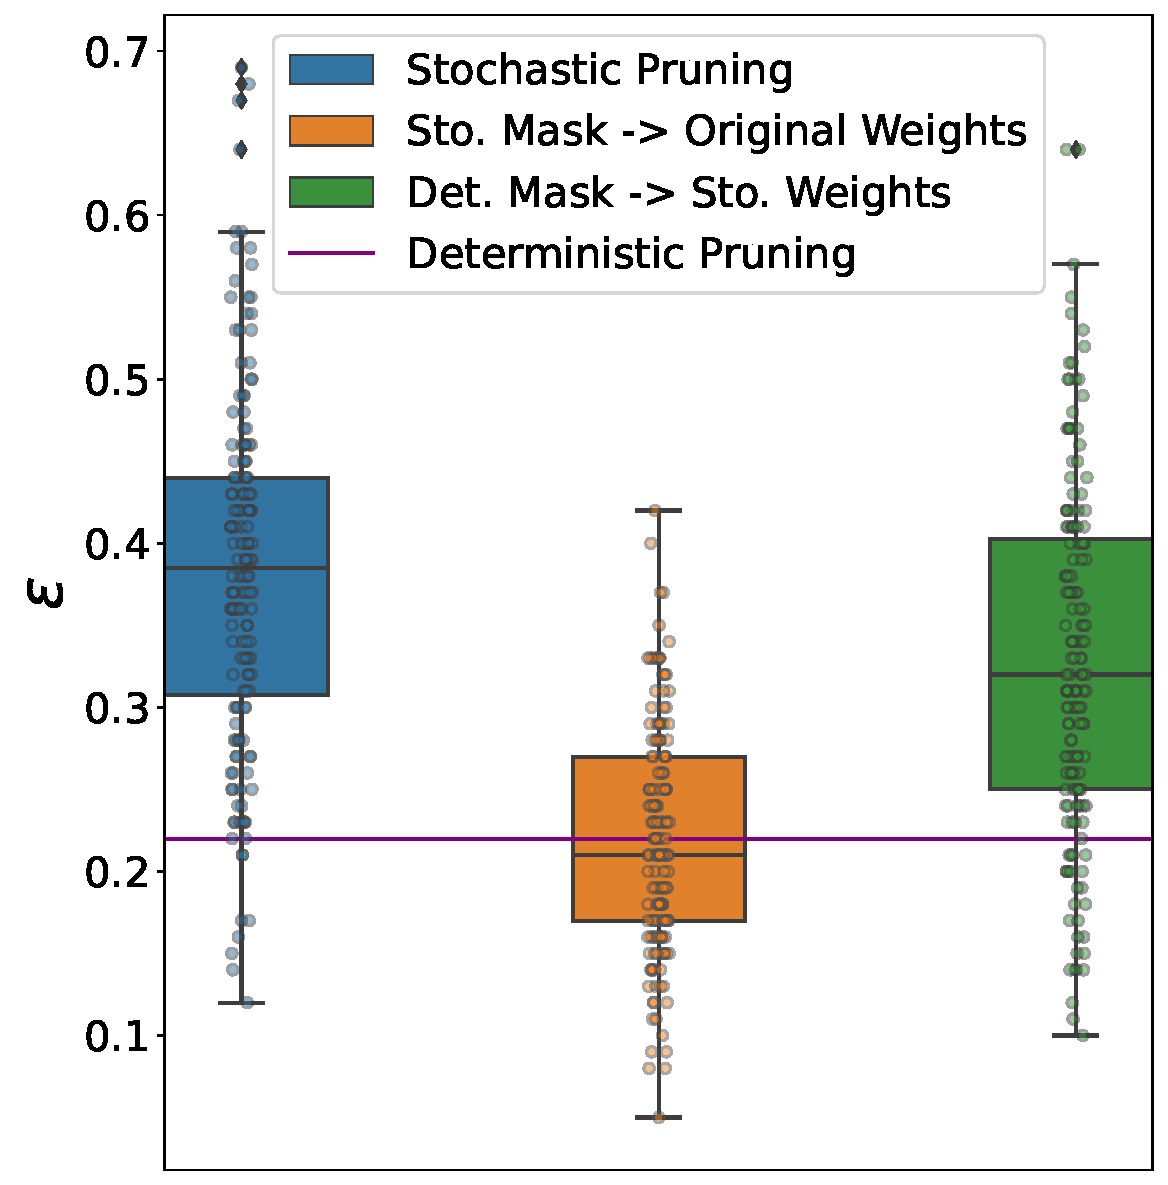
\includegraphics[width=\columnwidth]{figures/epsilon_allN_all_pr_0.5_sigma=0.003.pdf}
%     \caption{Accuracy degradation on CIFAR10 for one-shot Stochastic Pruning with $\sigma=0.003$ and pruning rate of 0.5} \label{fig:pr0.5sigma0.003}
%   \end{figure}%


%   \begin{figure}[htb]
%     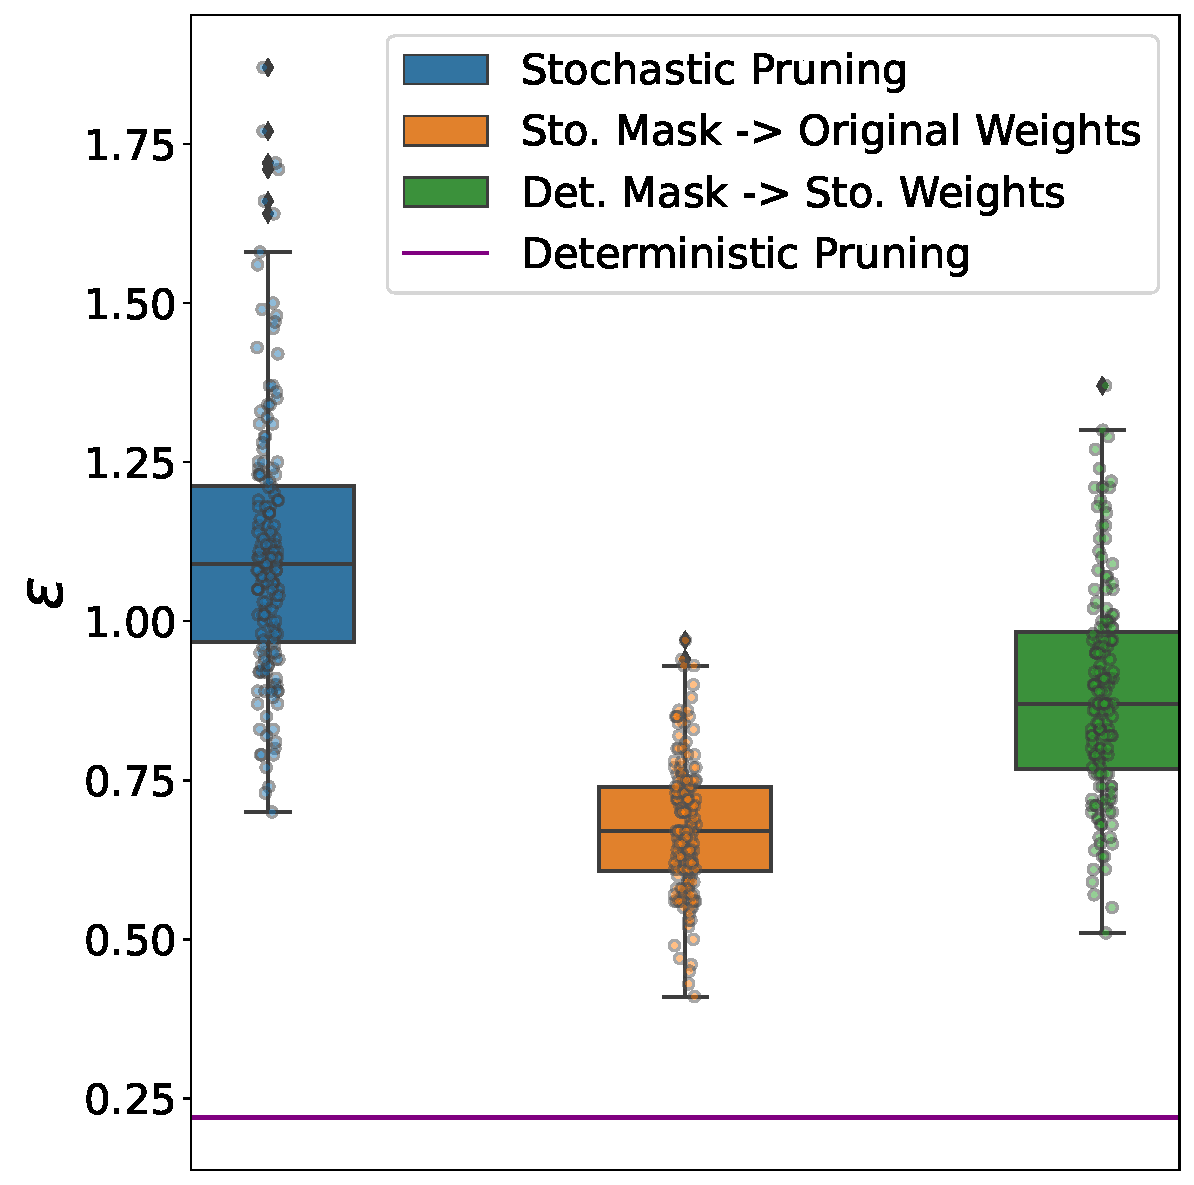
\includegraphics[width=\columnwidth]{figures/epsilon_allN_all_pr_0.5_sigma=0.005.pdf}
%     \caption{Accuracy degradation on CIFAR10 for one-shot Stochastic Pruning with $\sigma=0.005$ and pruning rate of 0.5} \label{fig:pr0.5sigma0.005}
%   \end{figure}%
%   \begin{figure}[htb]
%     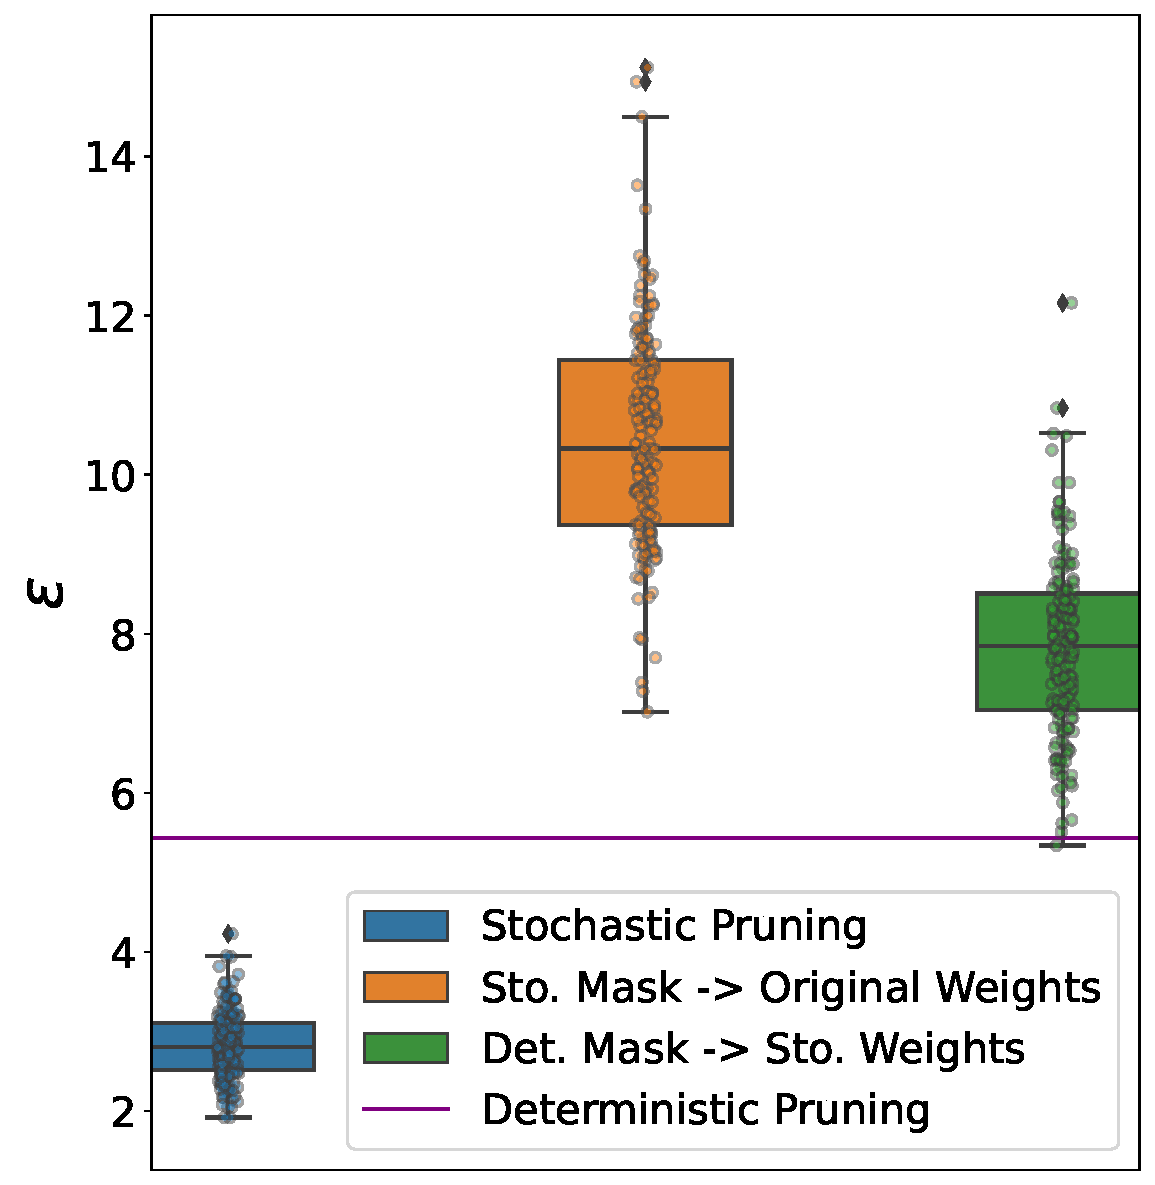
\includegraphics[width=\columnwidth]{figures/epsilon_allN_all_pr_0.8_sigma=0.005.pdf}
%     \caption{Accuracy degradation on CIFAR10 for one-shot Stochastic Pruning with $\sigma=0.005$ and pruning rate of 0.8} \label{fig:pr0.8sigma0.005}
%   \end{figure}%
%   \hspace*{\fill}   % maximizeseparation between the subfigures
%   \begin{figure}[htb]
%     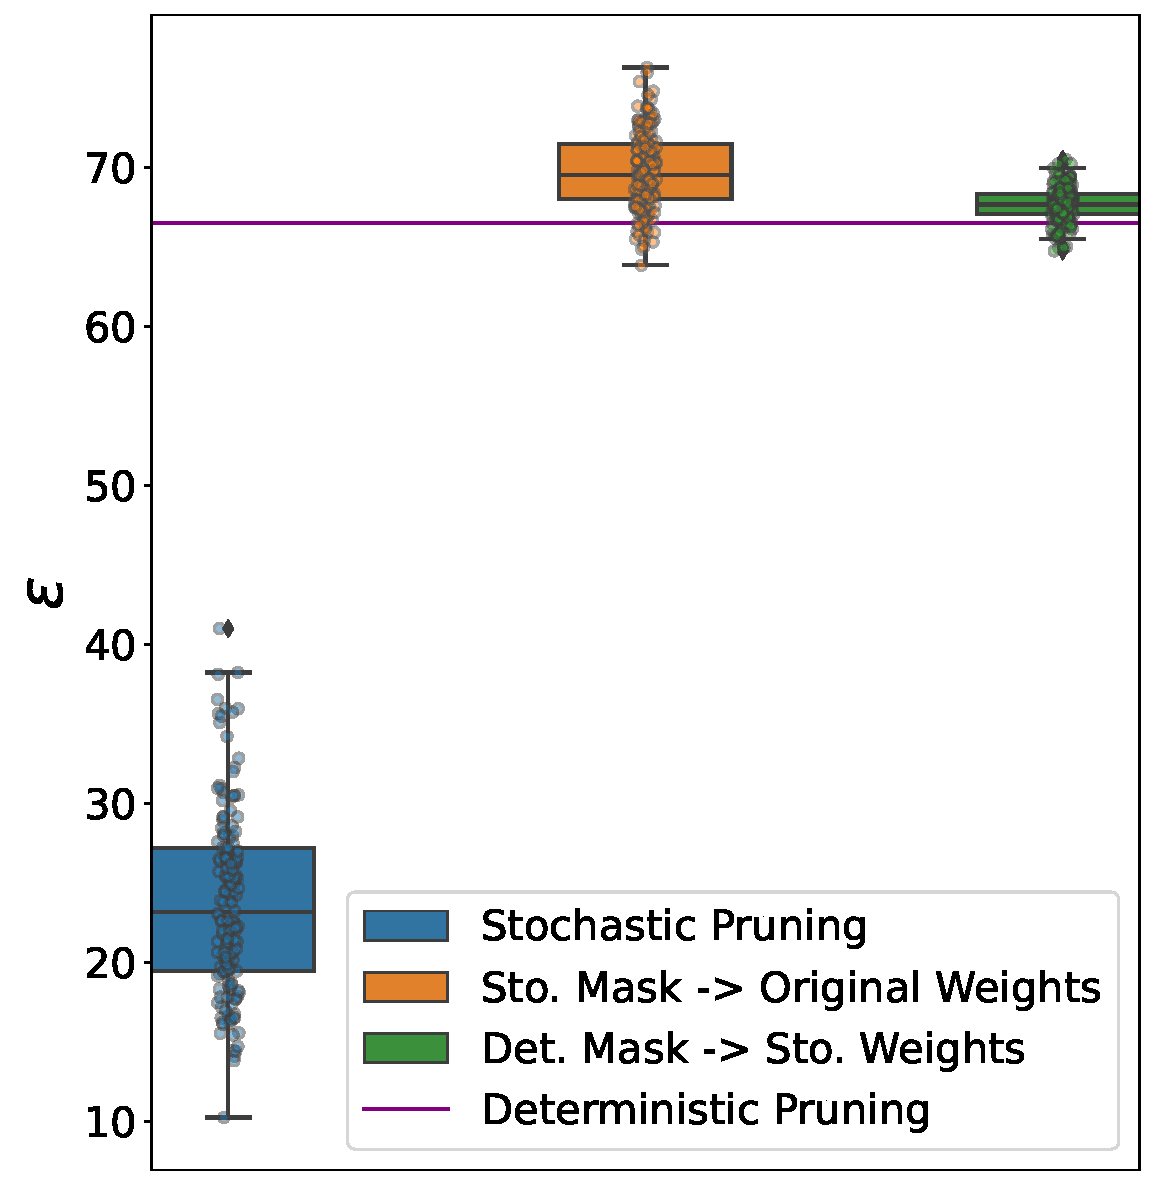
\includegraphics[width=\columnwidth]{figures/epsilon_allN_all_pr_0.9_sigma=0.005.pdf}
%     \caption{Accuracy degradation of Stochastic Pruning wit $\sigma=0.005$ and pruning rate of 0.9} \label{fig:pr0.9sigma0.005}
%   \end{figure}
% \subsection{Analysis of Stochastic Pruning per layer}

% It could be the case that  stochastic pruning does not affect  all layers equally and the experiments show here  will tell us, which layers are more affected by stochastic pruning and if we should normalise the noise amplitude for each layer separately, given the distribution of their weight's magnitude

% \begin{figure*}[tb]
%     \begin{subfigure}{}
%         \centering
%     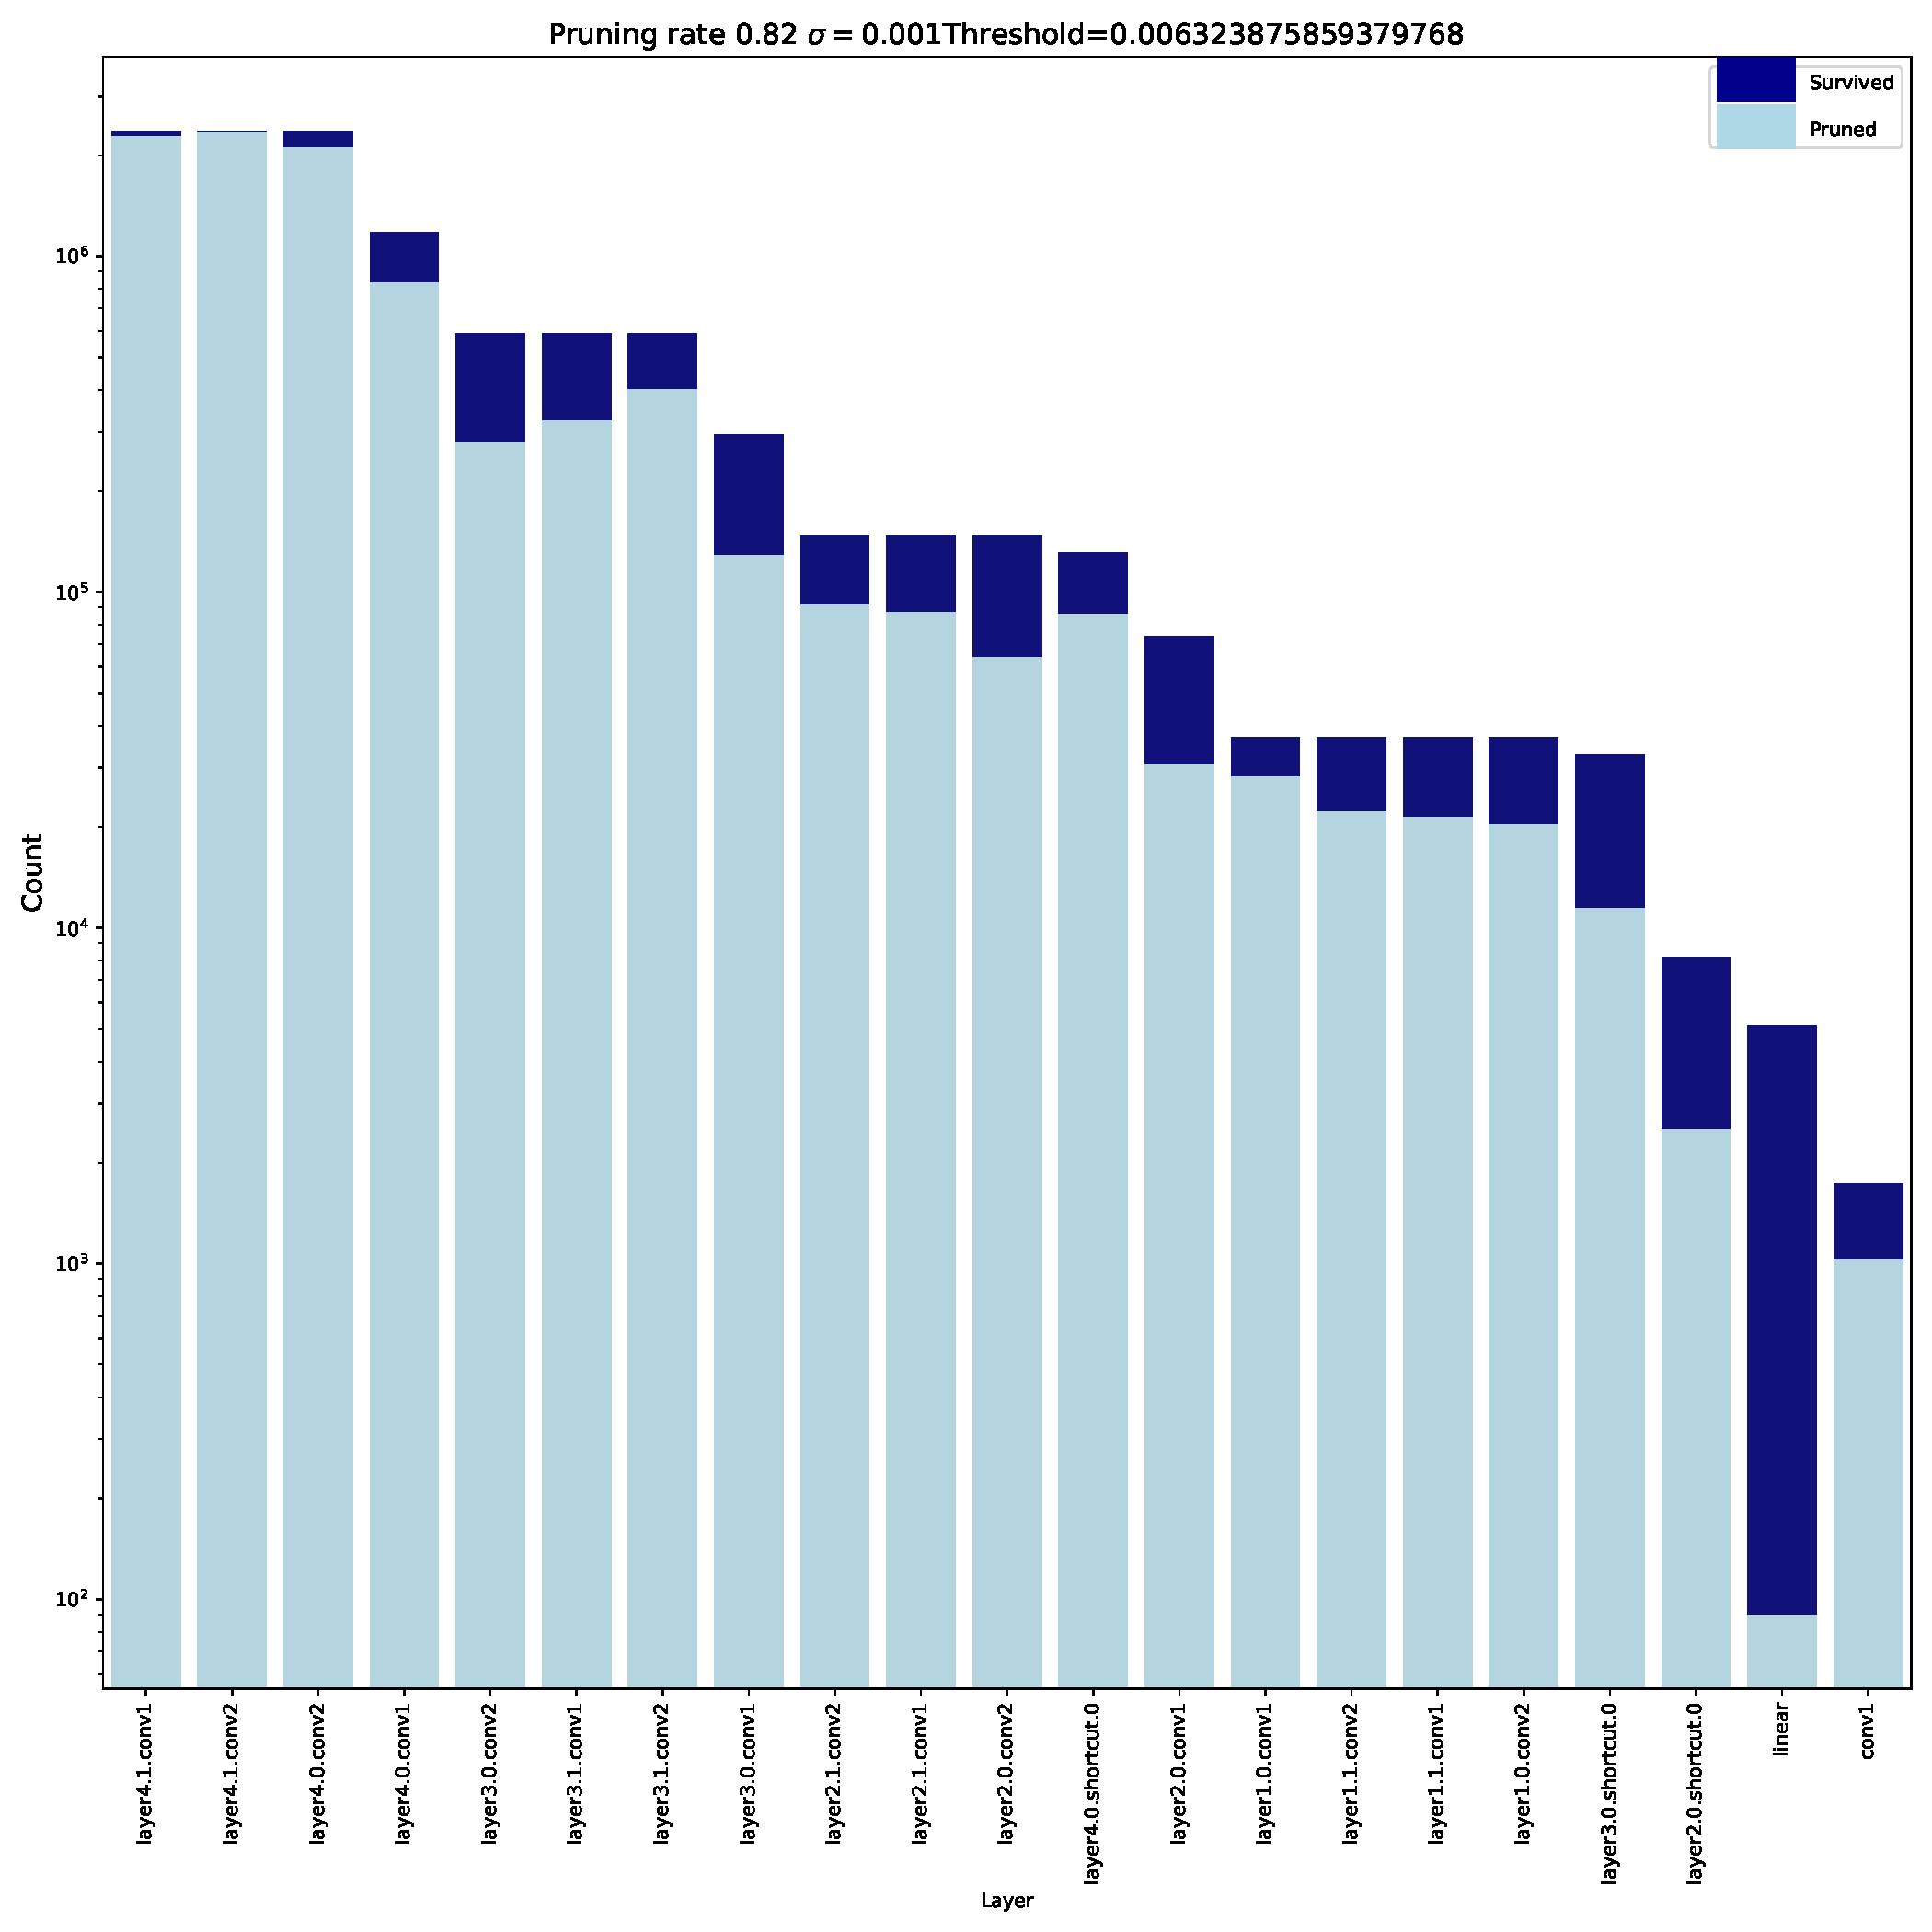
\includegraphics[width=0.2\textwidth]{supplementary/test_pr_0.82.pdf}
%     \caption{Remaining and pruned weights for pruning rate 82\%}
%     \label{subfig:pr_0.82}
%     \end{subfigure}
%     \begin{subfigure}{}
%     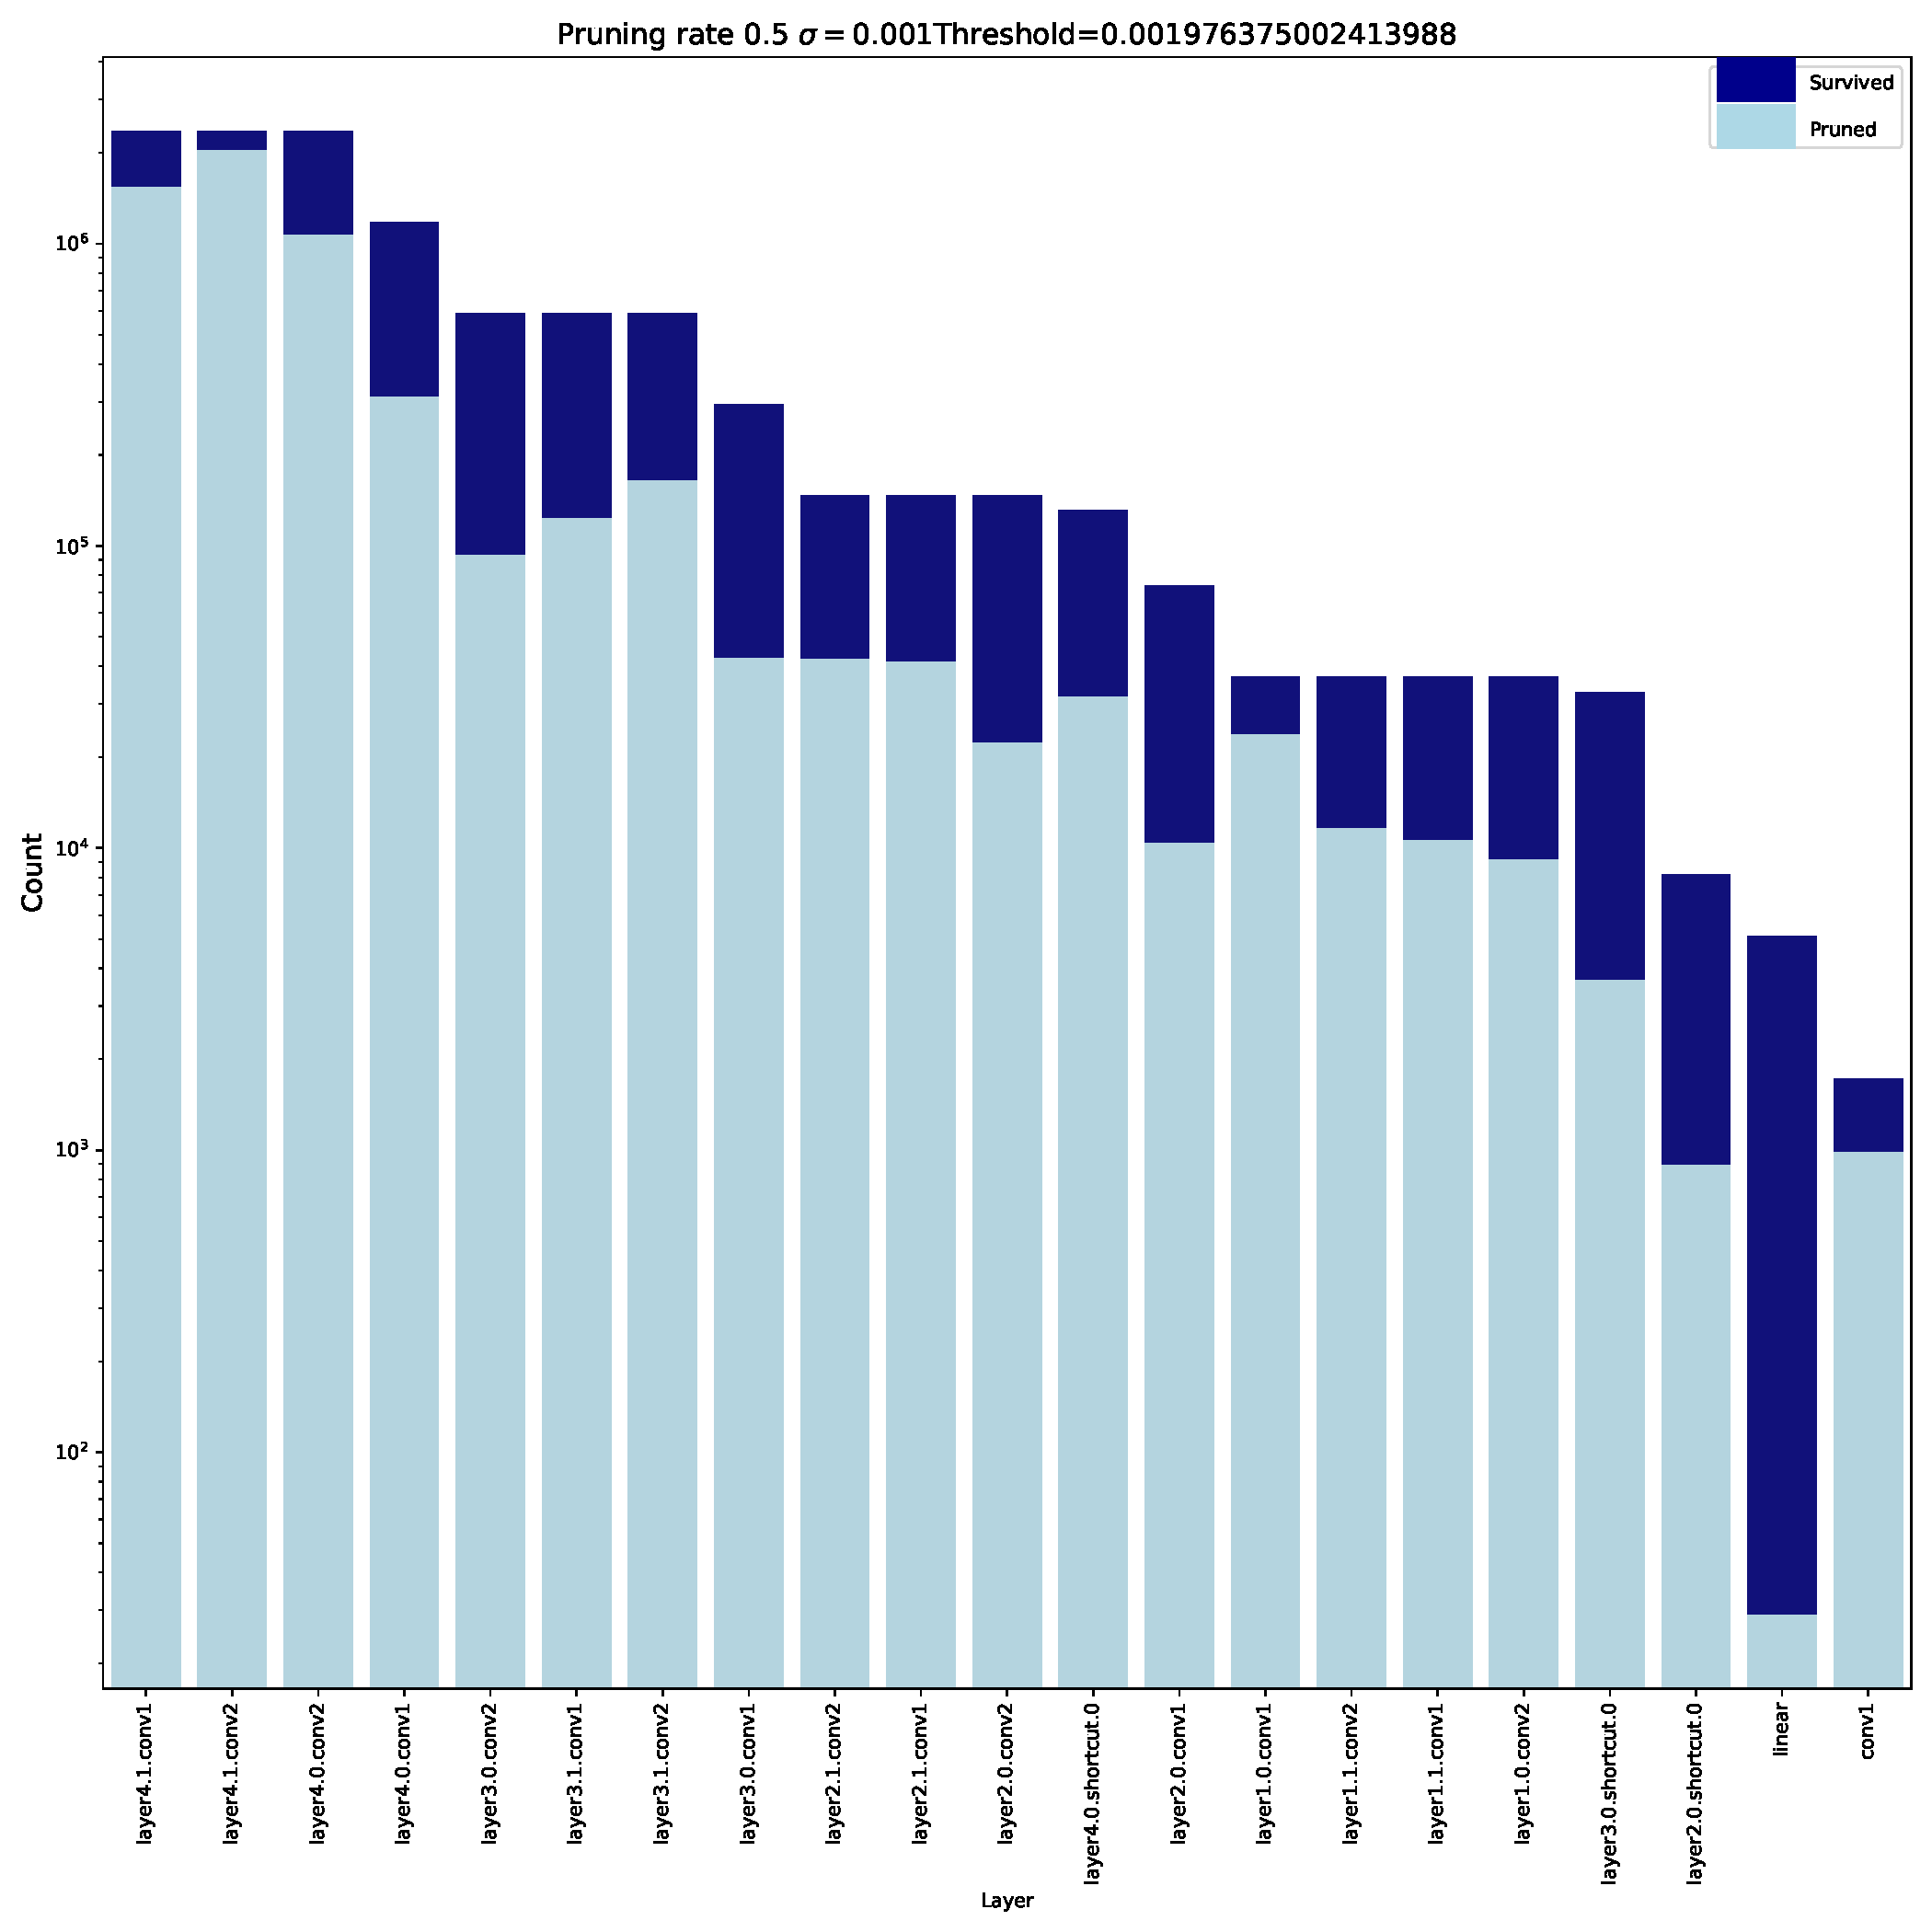
\includegraphics[width=0.2\textwidth]{supplementary/test_pr_0.5.pdf}
%     \label{subfig:pr_0.5}
%     \caption{Remaining and pruned weights for pruning rate 50\%}
%     \end{subfigure}
%     \begin{subfigure}{}
%     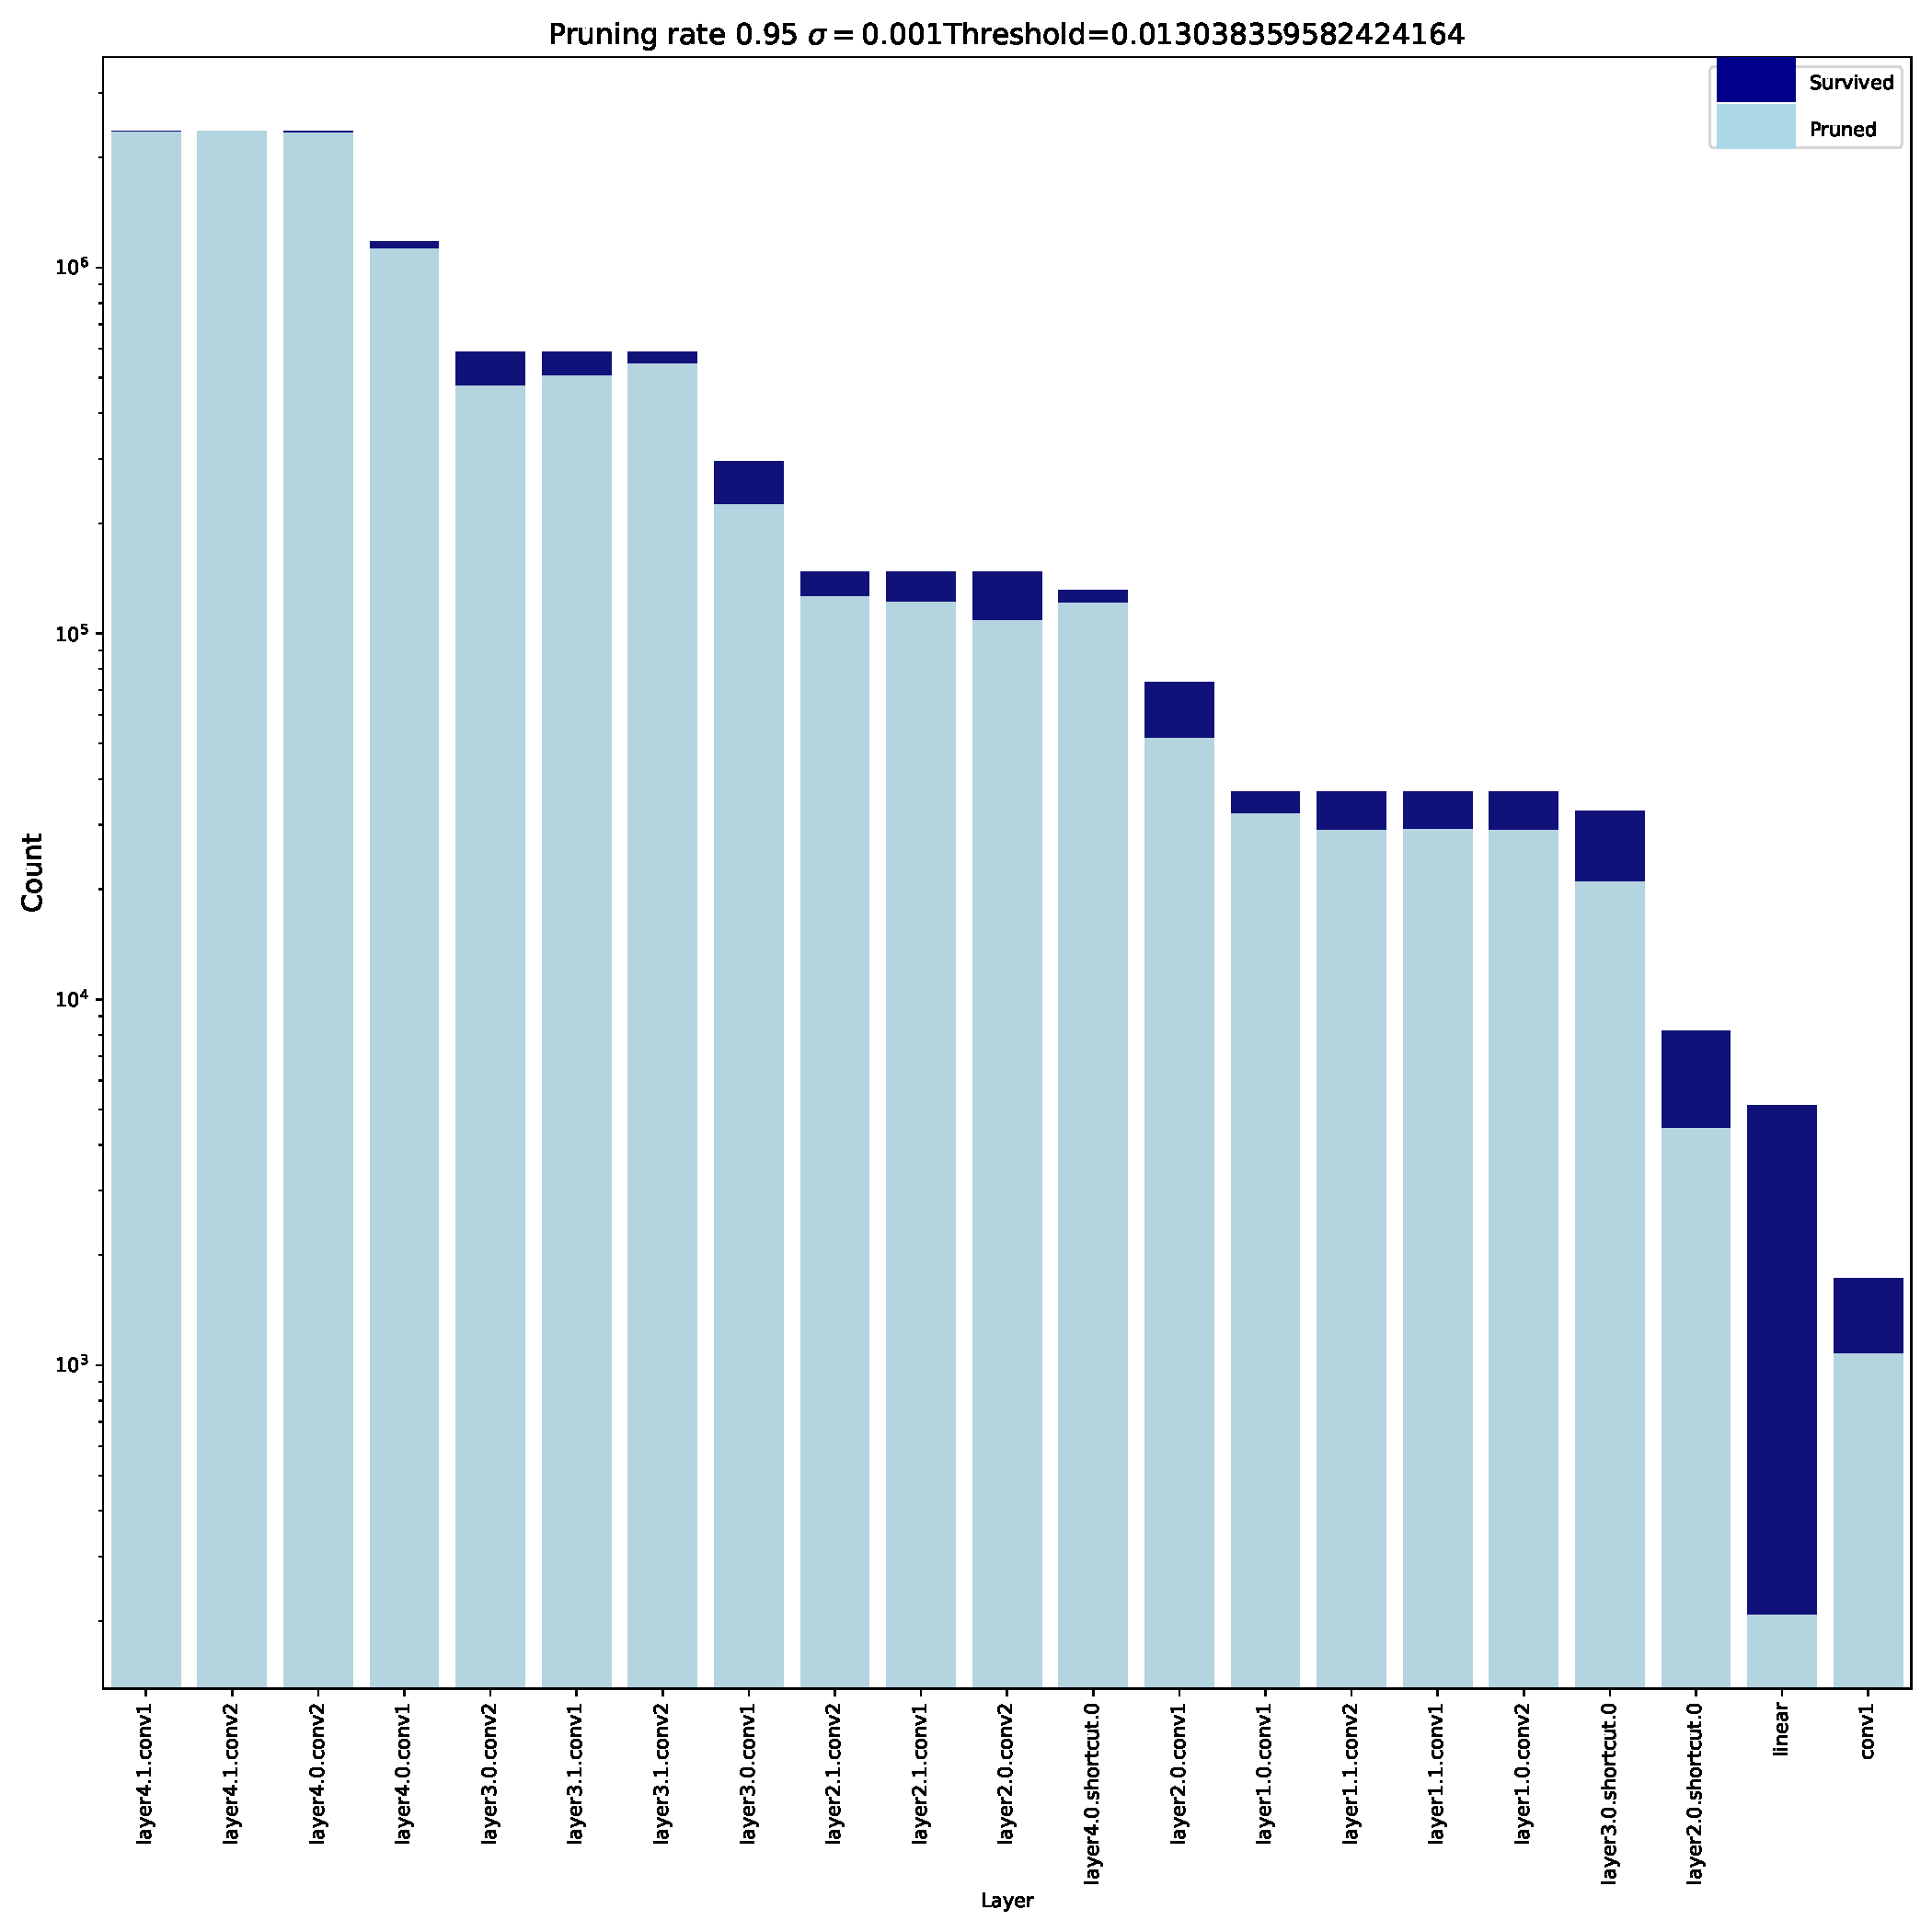
\includegraphics[width=0.2\textwidth]{supplementary/test_pr_0.95.pdf}
%     \caption{Remaining and pruned weights for pruning rate 95\%}
%     \label{subfig:pr_0.95}
%     \end{subfigure}
%     \hfill
%     \caption{Survival and pruned weights by layer}
% \end{figure*}
% Then
